%% Los cap'itulos inician con \chapter{T'itulo}, estos aparecen numerados y
%% se incluyen en el 'indice general.
%%
%% Recuerda que aqu'i ya puedes escribir acentos como: 'a, 'e, 'i, etc.
%% La letra n con tilde es: 'n.

\chapter{Transformación de Darboux}

La transformación de Darboux es una herramienta que permite construir una ecuación diferencial a partir de otra, con la principal característica que las soluciones de la nueva ecuación están dadas en función a las soluciones del sistema anterior. A continuación se muestra la deducción de esta herramienta.

\section{Esquema general}

Partiendo de la ecuación de Schrödinger independiente del tiempo y en unidades adecuadas ($\frac{\hbar}{2m}=1$)

\begin{equation}
\hat{H}\psi_E = E \psi\,\,\, : \,\,\,\hat{H} = -\frac{d^2}{dr^2}	+ V_0(r)  \label{SE-2}
\end{equation}

Si aplicamos un operador $\hat {D}$ a ambos lados de (\ref{SE-2})

\begin{equation*}
\hat{A}\hat{H}\psi_E = E \hat{A}\psi_E
\end{equation*}

podemos escribir el lado izquierdo de esta nueva ecuación en términos del conmutador de ambos operadores

\begin{equation}
  (\hat{H}\hat{A} - [\hat{H},\hat{A}])\psi_E = E \hat{A}\psi_E \label{nSE}
\end{equation}

El operador $\hat{A}$ de define en representación de coordenadas como

\begin{equation*}
	\hat{A} = \frac{d}{dr} - \beta(r)
\end{equation*}

por lo que el conmutador se puede escribir de la forma

\begin{equation*}
[\hat{H},\hat{A}] = \beta'' + 2 \beta' \frac{d}{dr} - V'_0.
\end{equation*}

Para escribir esta expresión en términos de $\hat{A}$, podemos sumar un cero de la forma

\begin{eqnarray*}
[\hat{H},\hat{A}] &=& \beta'' + 2 \beta' \frac{d}{dr} - 2\beta' \beta + 2\beta' \beta - V'_0.
\\
&=& (\beta' + \beta^2 - V_0)' + 2\beta' \hat{A}.
\end{eqnarray*}

Finalmente, la ecuación (\ref{nSE}) en términos de un nuevo hamiltoniano $\hat{H_1}$

\begin{equation}
\hat{H_1}\hat{A}\psi_E - (\beta' + \beta^2 - V_0)'\psi_E = E \hat{A}\psi_E \
\end{equation}

la cual tiene la forma de una ecuación de Scrödinger con potencial $V_1 = V_0 - 2 \beta'$ y soluciones $\hat{A} \psi_E$, siempre y cuando la siguiente condición se satisfaga

\begin{equation}
	\beta' + \beta^2 - V_0 = \epsilon. \label{RE}
\end{equation}

La expresión (\ref{RE}) es conocida como $"$Ecuación de Riccati $"$, que es una ecuación de segundo grado, y se puede linearizar proponiendo la siguiente forma para $\beta$

\begin{equation*}
\beta = \frac{u'}{u}
\end{equation*}

Finalmente, auatituyendo $\beta$ en la ecuación de Riccati, ésta es mapeada a una ecuación de Schrödinger con potencial $V_0$ y energía $\epsilon$.

\begin{equation*}
-u'' + V_0 u = \epsilon u
\end{equation*}

Esto quiere decir que mediante una solución partícular a una ecuación de Schrödinger con potencial $V_0$ podemos construir una nueva ecuación cuyo potencial y soluciones estarán dadas a partir de las sigientes relaciones

\begin{eqnarray}
\label{DT1-V}
V_1 &=& V_0 - 2 \frac{d^2}{dr^2} \ln \psi_\epsilon 
\\
\label{DT1-Psi}
\psi_E^{(1)} &=& \frac{W(\psi_\epsilon,\psi_E)}{\psi_\epsilon}.
\end{eqnarray}

La función $\psi_\epsilon$ se conoce como $"$Función de transformación$"$ o $"$función semilla $"$, mientras que $W(\cdot,\cdot)$ denota el wornskiano de dos funciones. Ya que la expresión para $\psi_E^{(2)}$ contiene a la función de transformación como denominador, es necesario que ésta no tenga ceros para evitar singularidades en las soluciones del nuevo sistema. Por lo tanto, sólo es posible usar el estado base o una solución no física, lo cual limita la usabilidad de la herramienta. A continuación se mostrará el uso de la herramienta aplicada tomando como sistema inicial el oscilador armónico unidimensional

\subsection{Ejemplo: Oscilador armónico}

Como sistema inicial, tomamos un oscilador armónico, descrito por la ecuación de Scrödinger

\begin{equation}
- \frac{d^2 \psi}{dx^2} + x^2 \psi = E\psi. \label{ES-OA}
\end{equation}

En este caso, $\frac{\hbar}{2m} = \frac{m\omega^2}{2} = 1$. Existen varias formas de resolver este sistema, tales como el método de factorización o el método de serie de potencias. Sin embargo, con el propósito de obtener una forma general para las soluciones, incluyendo las que no tienen un significado físico, se puede mapear (\ref{ES-OA}) a una ecuación hipergeométrica cuya solución general es

\begin{eqnarray*}
	\psi(x) &=& A \,_1 F_1 \left(a, \frac{1}{2},x^2 \right) e^{-\frac{x^2}{2}} +  B \,_1 F_1 \left(a + 1, \frac{3}{2}, x^2 \right) x e^{-\frac{x^2}{2}}
	\\
	a &=& \frac{1-E}{4}
\end{eqnarray*}

donde $\,_1 F_1$ es la función hipergeométrica dada en términos del símbolo de Pochhamer

\begin{equation*}
\,_1 F_1 \left(a,b,z\right) = \sum^\infty_{n=0}{\frac{(a)_n}{(b)_n} \frac{z^n}{n!}}, \,\,\, (a)_n = \prod_{k=0}^{n-1}{a+k}	
\end{equation*}


Por lo tanto, para obtener las soluciones con significado físico, es necesario truncar la función hipergeométrica, lo cual se logra a través de imponer que el primer argumento de la misma sea un número entero negativo $-n$. Ya que $a \ne a+\frac{1}{2}$, tenemos entonces dos casos

\begin{eqnarray*}
	\frac{1-E}{4} = -n \Rightarrow E = 4 n + 1
	\\
	\frac{3-E}{4} = -n \Rightarrow E = 4 n + 3
\end{eqnarray*}


lo que divide las soluciones en dos conjuntos de funciones con paridad definida

\begin{eqnarray*}
	\psi_e(x) &=& A \,_1 F_1 \left(-\frac{n}{2}, \frac{1}{2},x^2 \right) e^{-\frac{x^2}{2}}, \, n \, par
	\\
	\psi_o(x) &=&  B \,_1 F_1 \left(-\frac{n+1}{2}, \frac{3}{2}, x^2 \right) x e^{-\frac{x^2}{2}} \, n \, impar .
\end{eqnarray*}

El espectro de energía esta constituido por un conjunto de valores discretos dados por la regla de cuantización

\begin{equation*}
E = 2 n +1, \,\,\, n = 0,1,2,3,...
\end{equation*}

Una vez obtenido el conjunto de estados, podemos proceder a utilizar las fórmulas (\ref{DT1-V}) y (\ref{DT1-Psi}) para construir un nuevo sistema, empezando por utilizar el estado base como función de transformación, por lo que el potencial está dado por

\begin{equation*}
V^{(1)} = x^2 - 2 \frac{d^2}{dx^2} \ln(e^{\frac{-x^2}{2}}) = x^2 + 4.
\end{equation*}

Este no es más que el potencial de partida desplazado, por lo que es físicamente equivalente, por lo que este resultado no es de inerés.

Por otro lado, sí se usa como función de tramsformación una solución asociada a un eigenvalor $E$ menor al correspondiente al estado base, se observa que al transformar el estado base se obtiene una función con un nodo, lo que sugiere que el estado base del nuevo sistema se puede obtener a partir de una solución no física. Este tipo de estados son comúnmente llamados $"$missing states$"$, los cuales se pueden calcular a partir de asumir la ortogonalidad entre los estados ligados

\begin{equation*}
(\psi^{(1)}_m, \psi^{(1)}_E) = 0
\end{equation*}

donde $(\cdot , \cdot)$ denota el producto interno de dos funciones y $\psi^{(1)}_m$ es el missing state. Ya que sabemos que todos los demás estados están dados por la transformación de Darboux, entonces

\begin{equation*}
(\psi^{(1)}_m, \hat{A} \psi_E) = 0,
\end{equation*}

y como $\hat{A}$ es hermitiano

\begin{equation*}
(\hat{A}^\dagger \psi^{(1)}_m, \psi_E) = 0,
\end{equation*}

se concluye que la ecuación para obtener el missing state es

\begin{equation*}
\psi^{(1)}_m = \frac{1}{\psi_\epsilon},
\end{equation*}

La figura \ref{TD1OA-Figure} muestra un ejemplo de un sistema con un missing state.

\begin{figure}
	\centering
	\subfloat[]{%
		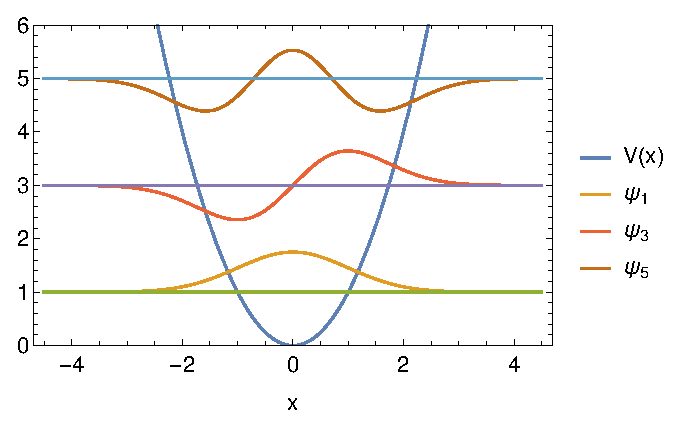
\includegraphics[width=0.47\textwidth]{OA-Fig.eps}%
		\label{fig:a}%
	}%
	\hfill%
	\subfloat[]{%
		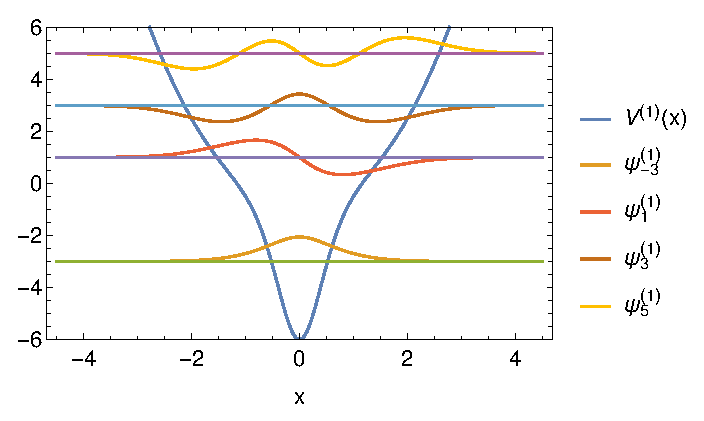
\includegraphics[width=0.47\textwidth]{TD1OA-Fig.eps}%
		\label{fig:b}%
	}%
	\caption{\label{TD1OA-Figure} (a) Oscilador armónico con sus estados correspondientes a los tres primeros niveles energéticos, el cual se toma como sistema inicial para construir (b), usando como función de tramsformación $\psi_e$ correspondiente a $E= -3$. Dicho sistema cuenta con un nivel energético extra, correspondiente al mismo eigen valor de la función de transformación.}
\end{figure}

La transformación de Darboux se puede aplicar de forma iterativa, lo que permite utilizar el resto de los estados como funciones semilla para la cinstrucción de nuevos sistemas. Este método es conocido como transformación de Darboux de orden superior, el cual se estudiará en la siguiente sección.
\section{Transformación de Darboux de orden superior}

Si tenemos un sistema dado por un potencial construido a partir de (\ref{DT1-V}) y lo usamos como punto de partida para aplicar nuevamente la transformación de Darboux, la función de semilla debe ser de la forma

\begin{equation*}
	\psi_T = \frac{W(\psi_{\epsilon_1},\psi_{\epsilon_2})}{\psi_{\epsilon_1}}.
\end{equation*}

De manera que el nuevo potencial estará dado por 

\begin{equation}
\label{TD2-V}
V^{(2)}=V^{(1)} - 2 \frac{d^2}{dr^2} \ln \psi_T = V_0 - 2  \frac{d^2}{dr^2} \ln [{W(\psi_{\epsilon_1},\psi_{\epsilon_2})}],
\end{equation}

mientras que las soluciones al nuevo sistema son obtenidas por medio de la relación

\begin{equation*}
\psi_E^{(2)} = \frac{\psi_{\epsilon_1}W \left[\frac{ W(\psi_{\epsilon_1},\psi_{\epsilon_2})}{\psi_{\epsilon_1}},\frac{W(\psi_{\epsilon_1},\psi_{E})}{\psi_{\epsilon_1}}\right]}{W(\psi_{\epsilon_1},\psi_{\epsilon_2})},
\end{equation*}

que se puede reducir por medio de las siguientes propiedades de los wronskianos

\begin{eqnarray*}
W[f(r)g(r),f(r)h(r)] &=& f^2(r) W[g(r),h(r)]
\\
W\{W[f(r),g(r)],W[f(r),h(r)]\} &=& f(r) W[f(r),g(r),h(r)].
\end{eqnarray*}

La expresión final queda entonces en función de dos funciones de transformación, las cuales son soluciones asociadas al potencial $V_0$

\begin{equation}
\label{TD2-Psi}
\psi_E^{(2)} = \frac{W(\psi_{\epsilon_1},\psi_{\epsilon_2},\psi_E)}{W(\psi_{\epsilon_1},\psi_{\epsilon_2})}.
\end{equation}

A diferencia de la transformación de Darboux de primer orden, en este caso tenemos que asegurar que el wornskiano de ambas funciones de transformación sea diferente de cero, lo que extiende la utilidad de la herramienta al permitirnos usar dos estados ligados del sistema inicial como funciones semilla. Sin embargo, los potenciales mostrados en la figura  \ref{TD2OA-Figure} sugieren que los mismos están libres de singularidades solo para el caso en que los niveles energéticos de las funciones de transformación sean contiguos, es decir $\epsilon_2 = \epsilon_1 + 2$ para el caso del oscilador armónico, tal como el sistema ilustrado en la figura \ref{TD2OA0-Figure}. En caso contrario, el potencial tendrá un número de singularidades igual a la $"$ distancia$"$ entre los niveles energéticos entre las funciones de transformación (véase figura \ref{TD2OA1-Figure}).

\begin{figure}
	\centering
	\subfloat[]{%
		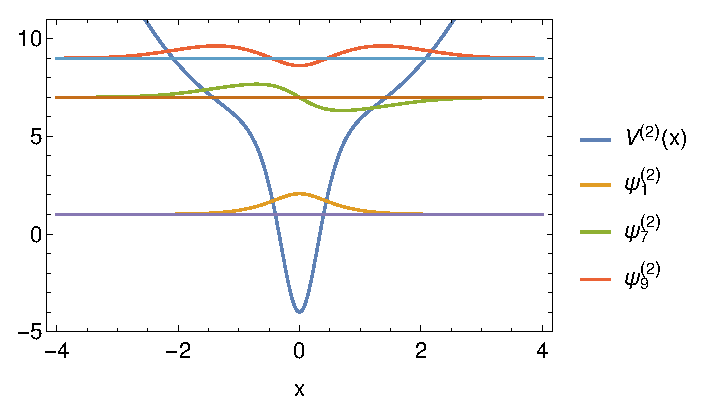
\includegraphics[width=0.47\textwidth]{TD2OA0-Fig.eps}%
		\label{TD2OA0-Figure:a}%
	}%
	\hfill%
	\subfloat[]{%
		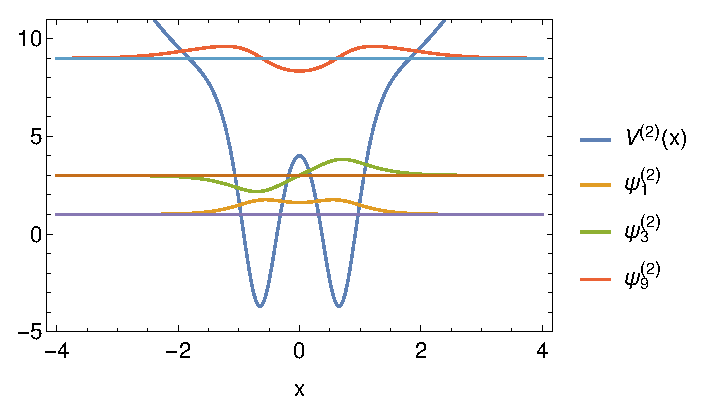
\includegraphics[width=0.47\textwidth]{TD2OA1-Fig.eps}%
		\label{TD2OA0-Figure:b}%
	}%
	\caption{\label{TD2OA0-Figure} Sistemas construidos a partir del oscilador armónico mostrado en la figura \ref{TD1OA-Figure} a través de la transformación de Darboux de segundo orden tomando como funciones de transformación  (a) el primero y segundo estado excitado, correspondientes a $\epsilon_1=3$, $\epsilon_2=5$ y  (b) el segundo y tercer estados exitados con $\epsilon_1=5$, $\epsilon_2=7$.
	 }
\end{figure}

\begin{figure}
	\hfill%
	\subfloat[]{%
		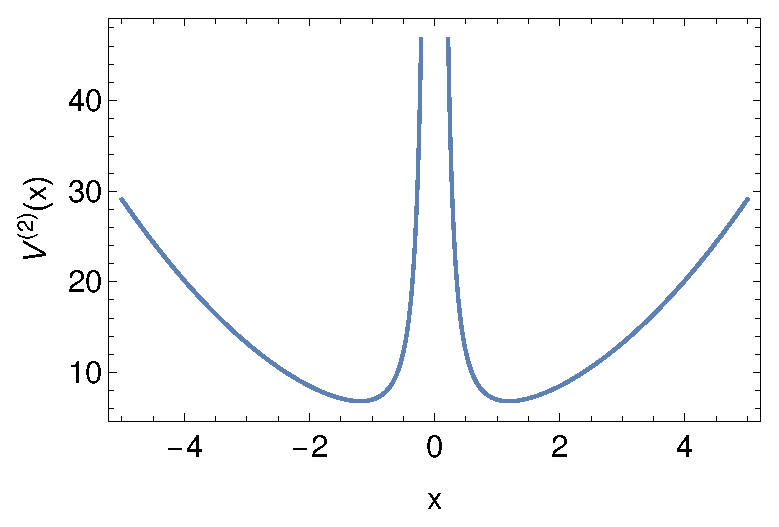
\includegraphics[width=0.47\textwidth]{TD2OA2-Fig.eps}%
		\label{TD2O1-Figure:a}%
	}%
	\hfill%
	\subfloat[]{%
		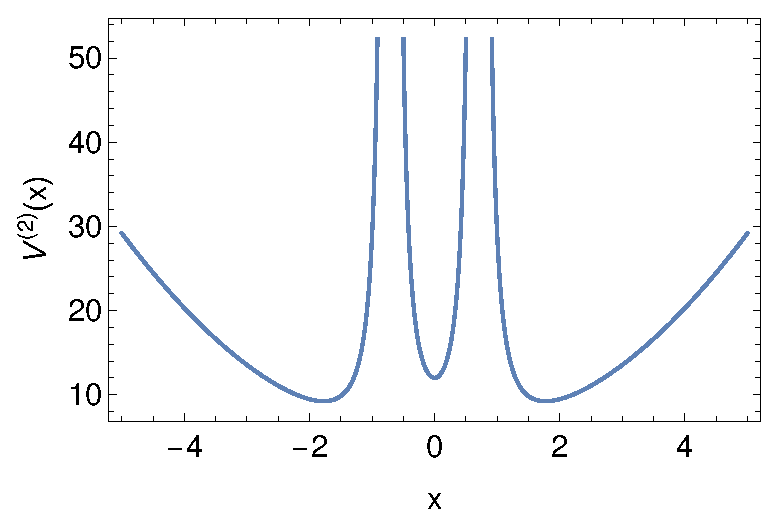
\includegraphics[width=0.47\textwidth]{TD2OA3-Fig.eps}%
		\label{TD2OA1-Figure:b}%
	}%
	\caption{\label{TD2OA1-Figure} Potenciales construidos a partir de la transformación de Darboux de segundo orden tomando como funciones semilla, las soluciones de cuadrado integrable correspondientes a (a) $\epsilon_1=1, \, \epsilon_2=5$ y (b) $\epsilon_1=1, \, \epsilon_2=7$. Para el caso de (a), existe un nivel de diferencia entre ambas funciones, el cual es $E=3$, por lo que el potencial resultante cuenta con una singularidad.
	}
\end{figure}

Es importante mencionar que ahora que tenemos dos funciones de transformación, en este caso puede ser posible la existencia de dos missing states, dependiendo de las funciones de transformación que se usen.

La transformación de Darboux se puede seguir aplicando de manera iterativa para obtener versiones de orden superior de esta herramienta, cuya generalización es conocida como transformación de Crum

\begin{eqnarray*}
	V^{(n)} = V_0 - 2 \frac{d^2}{dr}\ln[W(\psi_{\epsilon_1},...,\psi_{\epsilon_n})]
	\\
	\psi^{(n)} = \frac{W(\psi_{\epsilon_1},...,\psi_{\epsilon_n},\psi_E)}{W(\psi_{\epsilon_1},...,\psi_{\epsilon_n})}.
\end{eqnarray*}



Esta herramienta ha sido ampliamente estudiada para la construcción de sistemas por medio de la ingeniería de la parte discreta del espectro. Sin embargo, la transformación puede ser usada también en el regimen continuo con la adecuada modificación de la herramienta, proceso que se persentará en la siguiente sección.

\section{Transformación de Darboux degenerada}

En la subsección anterior, observamos como al usar la transformación de Darboux de segundo orden, el potencial resultante era no singular si las se usaban como funciones de transformación soluciones de cuadrado integrable (estados ligados), cuyos respectivos eigenvalores eran $"$ contiguos $"$. Siguiendo está idea, analizaremos lo que ocurre al construir un sistema por medio de la transformación de Darboux de segundo orden tomando dos soluciones de la dispersión cuyos valores sean contiguos, lo cual en el contexto continuo significa

\begin{equation*}
	\epsilon_2 = \epsilon_1 + \eta \,:\, |\eta|<<1.
\end{equation*}

Por lo que podemos expandir la solución $\psi_{\epsilon_2}$ en una serie de Taylor alrededor de $\epsilon_1$

\begin{equation*}
\psi(\epsilon_1 + \eta) = \psi(\epsilon_1) + \eta \partial_{\epsilon_1} \psi(\epsilon_1) + O(\eta^2).
\end{equation*}

Entonces las soluciones de un sistema dado por la transformación de Darboux de segundo orden están dadas por

\begin{equation*}
	\psi^{(2)} = \frac{W[\psi(\epsilon_1),\psi(\epsilon_1) + \eta \partial_{\epsilon_1} \psi(\epsilon_1) + O(\eta^2),\psi(E)]}{W[\psi(\epsilon_1),\psi(\epsilon_1) + \eta \partial_{\epsilon_1} \psi(\epsilon_1) + O(\eta^2)]}.
\end{equation*}

Gracias a la linealidad del wronskiano, podemos escribir numerador y denominador con $\eta$ como factor común

\begin{equation*}
\psi^{(2)} = \frac{\eta \{W[\psi(\epsilon_1), \partial_{\epsilon_1} \psi(\epsilon_1),\psi(E)] + W[\psi(\epsilon_1), O(\eta^2),\psi(E)]\}}{\eta\{W[\psi(\epsilon_1), \partial_{\epsilon_1} \psi(\epsilon_1)] + W[\psi(\epsilon_1), O(\eta^2)]\}},
\end{equation*}

para finalmete calcular el caso cuando $\eta \to 0$, lo que anula el segundo término en los corchetes tanto del numerador como del denominador

\begin{equation}
\psi^{(2)} = \frac{W[\psi(\epsilon_1), \partial_{\epsilon_1} \psi(\epsilon_1),\psi(E)]}{W[\psi(\epsilon_1), \partial_{\epsilon_1} \psi(\epsilon_1)]}, \label{TDD-Psi}.
\end{equation}

Siguiendo un procedimiento similar, se obtiene la fórmula para calcular el potencial deformado

\begin{equation}
V^{(2)} = V_0 - 2 \frac{d^2}{dr^2}\ln\{W[\psi(\epsilon_1), \partial_{\epsilon_1} \psi(\epsilon_1)]\}, \label{TDD-V2}.
\end{equation}

Es importante resaltar que el wronskiano sigue estando dado en términos de la posición, por lo que en las secciones restantes se volverá a usar la notación con sub indíces $\psi(E) = \psi_E$. Las fórmulas (\ref{TDD-Psi}) y $(\ref{TDD-V2})$ son equivalentes a realizar la transformación de Darboux de segundo orden con dos funciones semilla degeneradas, por lo que este esquema es conocido como transformación de Darboux con degeneración.

La herramienta construida a lo largo de esta sección será utilizada tomando como sistema de partida potenciales de corto alcance, ya que estos siempre cuentaan con un régiment de dispersión y cuyas generalidades se estudiarán en la siguiente sección.

